\documentclass[polish,polish,a4paper]{article}
\usepackage{cmap}

\usepackage[T1]{fontenc}
\usepackage[utf8]{inputenc}
\usepackage{listings}
\usepackage{graphicx} 
\usepackage{tikz}
\usepackage{xcolor}
\usepackage{babel}
\usepackage{pslatex}
\usepackage{tikz}
\usepackage{pgfplots}
\usepackage{anysize}
\usepackage{pgfgantt}
\usepackage{latexsym,amsmath}

\marginsize{2.5cm}{2.5cm}{3cm}{3cm}
\graphicspath{ {C:/Users/jankl/} }



\title{Sprawozdanie nr 1}
\author{Łukasz Szumilas}
\date{Zajęcia: 22 października 2018}

\begin{document}
  \begin{center}\Large
    Grafika Komputerowa i Komunikacja Człowiek-Komputer
  \end{center}
  \hrule
  {\let\newpage\relax\maketitle}
  \hrule


  \section{Omówienie tematu}
   Celem ćwiczenia jest zaprezentowanie elementarnych możliwości biblioteki graficznej OpenGL wraz z rozszerzeniem GL Utility Toolkit (GLUT). Ćwiczenie  obejmuje inicjalizację i zamykanie trybu OpenGL oraz rysowanie prymitywnych kształtów w przestrzeni 2D. 
   Pierwsza część to inicjalizacja szkieletu programu \textit{(Kod nr 1, Obraz nr 1)} wykorzystywanego później do rysowania figur.
(wzor ze strony: http://www.zsk.ict.pwr.wroc.pl)
\\\indent W drugiej części wystarczyło dodać dwie linijki \textit{(Kod nr 2, Obraz nr 2)} do funkcji \textit{RenderScene()}, by narysować niebieski kwadrat. 
\\\indent Przy zmianie zawartości funkcji \textit{RenderScene()}, które zostały uwzględnione w \textit{Kodzie nr 3}, ukazuje się dwukolorowy trójkąt \textit{Obraz nr 3}.
 \\\indent \textit{Kod nr 4}, pokazuje trójkolorowy trójkąt \textit{Obraz nr 4}.
\\\indent W ostatnim etapie należało napisać program tworzący \textbf{dywan sierpińskiego}. Algorytm dywanu: 
\begin{itemize}
\item  obiektem wyjściowym jest kwadrat o boku a,
\item  kwadrat dzielimy n 9 mniejszych równych kwadratów  o boku a/3 i  usuwamy środkow,
\item  każdy z mniejszych kwadratów  znów dzielimy na 9 części i  z każdej części usuwamy część środkową,
\item  powtarzmy dalsze kroki według wyżej opisanej zasady.
\end{itemize}
 Kod \textit{(Kod nr 5, Obraz nr 5 i 6)} posiada możliwość kierowania poziomem perturbacji i stopniem podziału kwadratów.

  \section{Omówienie kodu}
   \textbf{Kod 1}, po wywołaniu ukazuje się nam szkielet programu.  
{\small
\begin{lstlisting}[language=C++]
#include <windows.h>
#include <gl/gl.h>
#include <gl/glut.h>

// Funkcaja okreslajaca, co ma byc rysowane 
// (zawsze wywolywana, gdy trzeba przerysowac scene)
void RenderScene(void)
{
    glClear(GL_COLOR_BUFFER_BIT); 
   // Czyszczenie okna aktualnym kolorem czyszczacym

    glFlush();
   // Przekazanie polecen rysujacych do wykonania
}

// Funkcja ustalajaca stan renderowania
void MyInit(void)
{
   glClearColor(0.5f, 0.5f, 0.5f, 1.0f);
   // Kolor okna wnetrza okna - ustawiono na szary
}

// Glowny punkt wejscia programu. Program dziala w trybie konsoli
void main(void)
{
   glutInitDisplayMode(GLUT_SINGLE | GLUT_RGBA);
   // Ustawienie trybu wyswietlania
   // GLUT_SINGLE - pojedynczy bufor wyswietlania
   // GLUT_RGBA - model kolorow RGB

   glutCreateWindow("Pierwszy program w OpenGL");
   // Utworzenie okna i okreslenie tresci napisu w naglowku okna

   
   glutDisplayFunc(RenderScene);
   // Okreslenie, ze funkcja RenderScene bedzie funkcja zwrotna (callback)
   // Biblioteka GLUT bedzie wywolywala ta funkcje za kazdym razem, gdy
   // trzeba bedzie przerysowac okno

   MyInit(); 
   // Funkcja MyInit (zdefiniowana powyzej) wykonuje wszelkie 
   // inicjalizacje konieczne przed przystapieniem do renderowania
  
   glutMainLoop();
   // Funkcja uruchamia szkielet biblioteki GLUT
}

}
\end{lstlisting}
}
  \textbf{Kod 1}, po wywołaniu ukazuje się nam szkielet programu.  
{\small
\begin{lstlisting}[language=C++]
glColor3f(0.0f, 0.0f, 1.0f);
glRectf(-50.0f, 50.0f, 50.0f, -50.0f);
\end{lstlisting}
}

  \textbf{Kod 2}, użyty w RednerScene(), po wywołaniu ukazuje się niebieski kwadrat.  
{\small
\begin{lstlisting}[language=C++]
glColor3f(0.0f, 0.0f, 1.0f);
glRectf(-50.0f, 50.0f, 50.0f, -50.0f);
\end{lstlisting}
}

\textbf{Kod 3}, zmieniona funkcja RenderScene(), rysująca dwukolorowy trójkąt.  
{\small
\begin{lstlisting}[language=C++]
void RenderScene(void)
{
	glClear(GL_COLOR_BUFFER_BIT);
	// Czyszczenie okna aktualnym kolorem czyszczacym
	glColor3f(0.0f, 0.0f, 1.0f);
	// Ustawienie aktualnego koloru rysowania na niebieski

	glBegin(GL_TRIANGLES);
	// Narysowanie niebieskiego trojkata
	glVertex2f(0.0f, 0.0f);
	glVertex2f(0.0f, 50.0f);
	glVertex2f(50.0f, 0.0f);
	glEnd();

	glColor3f(0.0f, 1.0f, 0.0f);
	// Ustawienie aktualnego koloru rysowania na zielony
	glBegin(GL_TRIANGLES);
	// Narysowanie zielonego trojkata
	glVertex2f(0.0f, 0.0f);
	glVertex2f(0.0f, 50.0f);
	glVertex2f(-50.0f, 0.0f);
	glEnd();
	glFlush();
	// Przekazanie polecen rysujacych do wykonania
}
\end{lstlisting}
}

\textbf{Kod 4}, zmieniona funkcja RenderScene(), rysująca trójkolorowy trójkąt.  
{\small
\begin{lstlisting}[language=C++]
void RenderScene(void)
{

	glClear(GL_COLOR_BUFFER_BIT);
	glBegin(GL_TRIANGLES);

	glColor3f(1.0f, 0.0f, 0.0f); // wierzcholek czerwony
	glVertex2f(-50.0f, 0.0f);
	glColor3f(0.0f, 1.0f, 0.0f); // wierzcholek zielony
	glVertex2f(0.0f, 50.0f);
	glColor3f(0.0f, 0.0f, 1.0f); // wierzcholek niebieski
	glVertex2f(50.0f, 0.0f);
	glEnd();

	glFlush();

}
\end{lstlisting}
}

\textbf{Kod 5}, gotowy program zawierający implementację dywanu Sierpińskiego wraz z manipulacją ustawień.
{\small
\begin{lstlisting}[language=C++]

#include <Windows.h>
#include <GL\glew.h>
#include <GL\freeglut.h>
#include <iostream>

using namespace std;
typedef float point2[2]; //punkt w przestrzeni do rysowania kwadratow

float width = 200; //szerokosc kwadratu
int level = 3; //stopien podzialu dywanu
float defLevel = 0; //stopien perturbacji


void DrawCarpet(float x, float y, float w)
{
	point2 a = { x, y }; //definiowanie punktow w przestrzeni
	float width = w;
	int i = 0;

	point2 b = { (a[0] + width + ((rand() % 100)*defLevel)), 
	(a[1] + ((rand() % 100)*defLevel)) };
	point2 c = { (a[0] + width + ((rand() % 100)*defLevel)), 
	(a[1] + width + ((rand() % 100)*defLevel)) };
	point2 d = { (a[0] + ((rand() % 100)*defLevel)), 
	(a[1] + width + ((rand() % 100)*defLevel)) };

	//tworzenie obiektu typu Polygon
	glBegin(GL_POLYGON);
	glVertex2fv(a);
	glVertex2fv(b);
	glVertex2fv(c);
	glVertex2fv(d);
	glEnd();

	//nastepny poziom w ktorym bedziemy definiowac obiekty typu Polygon, trzy razy mniejsze
	if (i > 0)
	{
		width = width / 3;
	}
}

void DrawAll(float x, float y, float width, int level)
{
	if (level > 0)
	{
	//funkcja wykorzystujaca rekurencje, poki poziom podzialu dywanu nie zejdzie do 0
	width = width / 3;
	glColor3f(((rand() % 100)*0.01), ((rand() % 100)*0.01), ((rand() % 100)*0.01));
	DrawAll(x, y, width, level - 1);
	glColor3f(((rand() % 100)*0.01), ((rand() % 100)*0.01), ((rand() % 100)*0.01));
	DrawAll(x + width, y, width, level - 1);
	glColor3f(((rand() % 100)*0.01), ((rand() % 100)*0.01), ((rand() % 100)*0.01));
	DrawAll(x + width + width, y, width, level - 1);
	glColor3f(((rand() % 100)*0.01), ((rand() % 100)*0.01), ((rand() % 100)*0.01));
	DrawAll(x, y + width, width, level - 1);

	glColor3f(((rand() % 100)*0.01), ((rand() % 100)*0.01), ((rand() % 100)*0.01));
	DrawAll(x + width + width, y + width, width, level - 1);
	glColor3f(((rand() % 100)*0.01), ((rand() % 100)*0.01), ((rand() % 100)*0.01));
	DrawAll(x, y + width + width, width, level - 1);
	glColor3f(((rand() % 100)*0.01), ((rand() % 100)*0.01), ((rand() % 100)*0.01));
	DrawAll(x + width, y + width + width, width, level - 1);
	glColor3f(((rand() % 100)*0.01), ((rand() % 100)*0.01), ((rand() % 100)*0.01));
	DrawAll(x + width + width, y + width + width, width, level - 1);
	}

	else
	{
		DrawCarpet(x, y, width);
	}

}


void RenderScene(void)
{
	glClear(GL_COLOR_BUFFER_BIT);
	DrawAll(-100, -100, width, level);
	glFlush();
}


void MyInit(void)
{
	glClearColor(0.5f, 0.5f, 0.5f, 1.0f);
}


void ChangeSize(GLsizei horizontal, GLsizei vertical)
{

	GLfloat AspectRatio;

	if (vertical == 0)
		vertical = 1;


	glViewport(0, 0, horizontal, vertical);
	glMatrixMode(GL_PROJECTION);

	glLoadIdentity();

	AspectRatio = (GLfloat)horizontal / (GLfloat)vertical;

	if (horizontal <= vertical)
		glOrtho(-100.0, 100.0, -100.0 / AspectRatio, 100.0 / AspectRatio, 1.0, -1.0);
	else
		glOrtho(-100.0*AspectRatio, 100.0*AspectRatio, -100.0, 100.0, 1.0, -1.0);

	glMatrixMode(GL_MODELVIEW);
	glLoadIdentity();

}

void main(int argc, char* argv[])

{
	do
	{
		cout << "Podaj stopien podzialu dywanu [1; 5] : " << endl;
		cin >> level;
		cout << level << endl;
	} while (level > 5 || level < 1);


	do
	{
		cout << "Podaj poziom perturbacji [0; 0.1] : " << endl;
		cin >> defLevel;
		cout << defLevel << endl;
	} while (defLevel > 0.1);

	glutInit(&argc, argv);

	glutInitDisplayMode(GLUT_SINGLE | GLUT_RGBA);

	glutCreateWindow("Drugi program w OpenGL");
	glutDisplayFunc(RenderScene);
	glutReshapeFunc(ChangeSize);
	MyInit();
	glutMainLoop();

	system("pause");
}
\end{lstlisting}
}
  \section{Rezultat prac}

    \begin{figure}[h!]
      \centering
      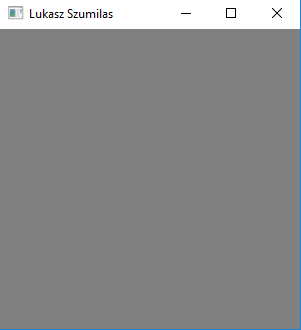
\includegraphics[width=0.6\textwidth,height=10cm]{empty.png}
      \caption{Szkielet biblioteki GLUT}
      \label{fig:zrzut1}
    \end{figure}
    
        \begin{figure}[h!]
      \centering
      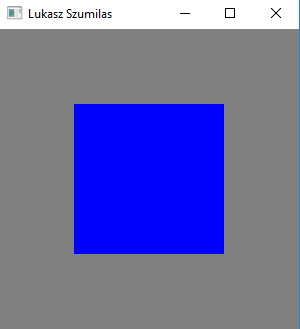
\includegraphics[width=0.6\textwidth,height=10cm]{kwadrat.png}
      \caption{Niebieski kwadrat}
      \label{fig:zrzut1}
    \end{figure}
    
            \begin{figure}[h!]
      \centering
      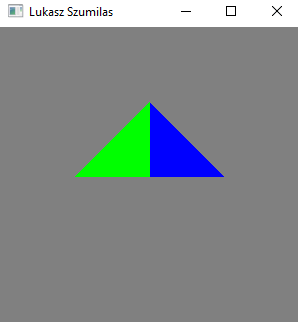
\includegraphics[width=0.6\textwidth,height=10cm]{trojkat.png}
      \caption{Dwukolorowy trójkąt}
      \label{fig:zrzut1}
    \end{figure}
    
      \begin{figure}[h!]
      \centering
      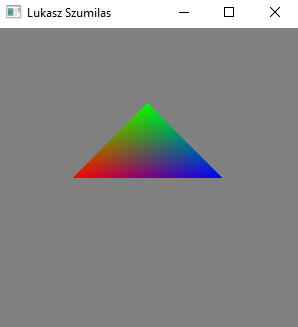
\includegraphics[width=0.6\textwidth,height=10cm]{trzykolory.png}
      \caption{Trójkolorowy trójkąt}
      \label{fig:zrzut1}
    \end{figure}
    
                \begin{figure}[h!]
      \centering
      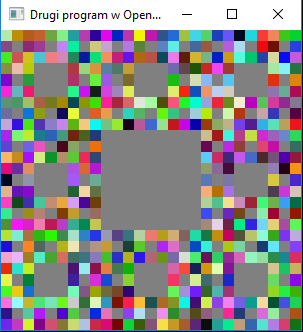
\includegraphics[width=0.6\textwidth,height=10cm]{dywan1.png}
      \caption{Dywan, stopien podzialu dywanu: 3. Poziom perturbacji: 0}
      \label{fig:zrzut1}
    \end{figure}
    
      \begin{figure}[h!]
      \centering
      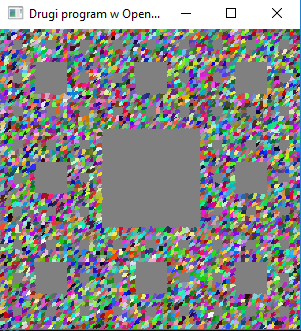
\includegraphics[width=0.6\textwidth,height=10cm]{dywan2.png}
      \caption{Dywan, stopien podzialu dywanu: 4. Poziom perturbacji: 0.05}
      \label{fig:zrzut1}
    \end{figure}

\end{document}